%%%%%%%%%% %%%%%%%%%% %%%%%%%%%%

% Purpose of the chapter
In this thesis we have made improvements to the search for \gws using a detector characterisation context by improving the quality of the detector data and understanding the noise background of the detectors. 

% Section by section of chapter
This chapter is laid out as follows: we briefly repeat our the state of the current \gwadj detector network in section~\ref{3:sec:gw_detectors}, in section~\ref{3:sec:detchar_calib} we define the research area of detector characterisation, the systematic sources of noise faced in the detectors is described in section~\ref{3:sec:detector-analysis}, some commonly detector data noise transients in section~\ref{3:sec:noise-transients} and finally, the detector characterisation tools most commonly used and referred to throughout this thesis in section~\ref{3:sec:detchar-tools}.

\section{\label{3:sec:gw_detectors}\Gwadj detectors}

% To understand the importance of Detector Characterisation we must understand the detectors
\Gwadj astronomy in the present day is performed by ground-based detectors at different locations globally: the LIGO-Livingston and LIGO-Hanford detectors are located in the United States of America, the Virgo interferometer in Italy and, the KAGRA telescope in Japan. We will primarily reference the LIGO detectors in the United States of America when discussing the challenges faced in detector characterisation. 

As described in chapter~\ref{chapter:1-gravitational-waves}, the LIGO detectors work on the principle of laser interferometry to detect \gwadj signals. The sensitivity~\cite{aLIGO_design_curve:2018} of \gwadj detectors is limited by fundamental sources of noise such as seismic noise~\cite{Glanzer:2023}, thermal noise~\cite{thermal_noise:2018} and quantum noise~\cite{quantum_noise:2003}. These are the non-stationary sources of noise~\cite{PSD_var:2020}. Additionally, we have non-Gaussian noise~\cite{Noise_Guide:2020} which manifests as transient noise bursts in the data which can contribute to false positives in \gwadj searches and the obscuring of real \gwadj signals~\cite{GW170817:2017, GW150914_noise:2016}.

\section{\label{3:sec:detchar_calib}Detector Characterisation and Calibration}

Detector characterisation is a field of study which assess and improves the performance of \gwadj detectors to ensure accurate and reliable detection of \gws. \Gwadj detector calibration determines how the response of the detector translates to astrophysical signals, ensuring accuracy in extracted astrophysical information. Detector characterisation is responsible for identifying and mitigating the many sources of noise that can obscure or mimic real signals. The optimisation of detector sensitivity is also studied whereby different designs and components can be fine-tuned to increase sensitivity. Another responsibility of detector characterisation is the monitoring of detector performance in real-time to assess sensitivity changes.

Overall, effective detector characterisation ensures that \gwadj observatories can operate at maximum potential and provide accurate and reliable observations of \gws. The \gwadj detector organisations have dedicated working groups for detector characterisation and calibration~\cite{O2O3_DetChar:2021, VirgoDetChar:2023}. In this thesis, chapter~\ref{chapter:4-archenemy} is a direct contribution to the field of detector characterisation with a contribution to the LIGO detector characterisation working group.

The detector characterisation group has the important task of verifying data quality when a \gwadj signal is detected by live detection pipelines, giving the confirmation that the \gwadj signal isn't a false alarm potentially caused by noise transients or poor data quality immediately surrounding the \gwadj signal.

\subsection{\label{3:sec:detector-analysis}Detector Analysis}

% Noise analysis
%    Different sources of noise
%    Seismic, thermal, shot, radiation pressure
%    Noise Curve

Systematic sources of noise are the dominating limit in the sensitivity of ground-based detectors. The sources of noise with the greatest contributions are
%
\begin{itemize}
    \item Seismic noise~\cite{Glanzer:2023}: the vibrations of the ground causes a coupled vibration motion in the mirrors of the interferometer. Higher frequency seismic noise ($1-10$Hz) is often caused by local ground movements typically anthropomorphic in nature or greater magnitude earthquakes~\cite{Nuttall:2018}. Lower frequency seismic noise ($<1$Hz) is caused by larger-scale geophysical processes such as: ocean waves, tidal effects, or smaller local earthquakes~\cite{aLIGO:2015}. Seismic noise can be mitigated with advanced suspension systems to isolate mirrors and end-station components from the ground to prevent coupling to seismic motion~\cite{seismic_isolation:2015}.
    \item Thermal noise~\cite{thermal_noise:2018}: the thermal energy of interferometer components will cause them to vibrate. This noise can be reduced with new mirror materials with resonant frequencies outside the sensitive regions or with cryogenically cooled mirrors such as those used by KAGRA~\cite{KAGRA:2021}.
    \item Shot noise~\cite{quantum_noise:2003}: the distribution in the number of photons observed by the interferometer photodetector in any time interval is Poisson distributed and the error in the photon count places limits on the sensitivity. The error is proportional to the square-root of the count ($\sigma \propto \sqrt{\lambda}$) therefore, the simplest way to reduce this error is to increase the laser power and increase the photon count in the time interval.
    \item Radiation pressure~\cite{quantum_noise:2003}: the pressure exerted by the photons hitting the end mirrors will decrease search sensitivity. To reduce this noise the laser power can be reduced however, this will increase the shot noise.
\end{itemize}

It can be seen that the laser power must be calibrated to balance the impact of increasing the photon count which will decrease shot noise but simultaneously increase radiation pressure noise. A figure displaying these systematic noise sources and their limitations in the LIGO detector case can be seen in figure~\ref{3:fig:aLIGO_noise}.
%
\begin{figure}
    \centering
    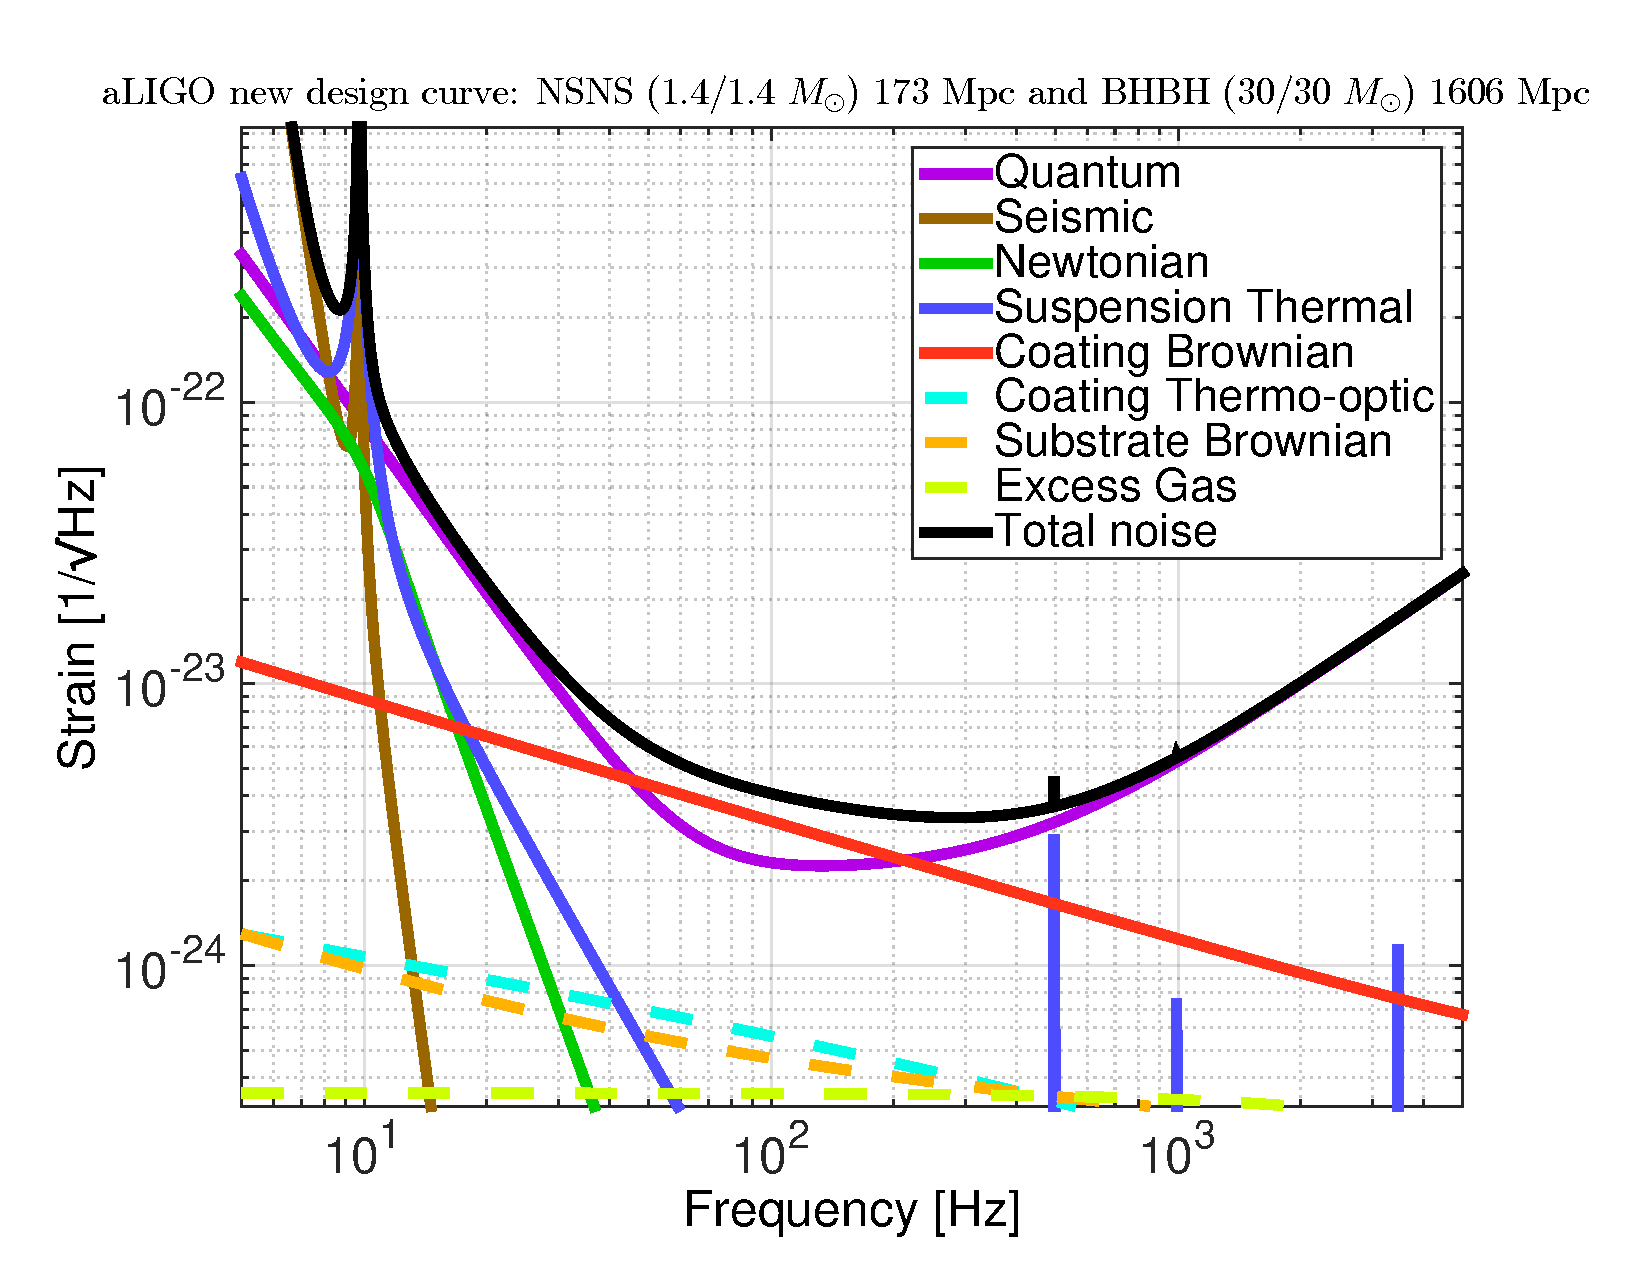
\includegraphics[width=0.75\linewidth]{images/3_detector_characterisation/aLIGO_newDesign.pdf}
    \caption{The Advanced LIGO~\cite{aLIGO:2015} strain sensitivity as a function of frequency (black solid line), accompanied by the systematic noise sources which limit the sensitivity of the detector. Taken from~\cite{aLIGO_design_curve:2018}.}
    \label{3:fig:aLIGO_noise}
\end{figure}
%

% Sensitivity Analysis
%    BNS Distance
%    Sensitivity Measurement
To monitor detector sensitivity the binary neutron star inspiral range is calculated. This is the range at which (in Mpc) a binary neutron star signal, with both components having a mass of $1.4$ M$_{\odot}$, will be detected given the characteristic noise (PSD) of the data. The PSD is calculated by taking an average of the detector noise in the previous minute~\cite{range_calculation:2003, ota:2023}. Figure~\ref{3:fig:bns_range} shows an example of the binary neutron star range for a day of LIGO-Hanford during the fourth observing run.
%
\begin{figure}
    \centering
    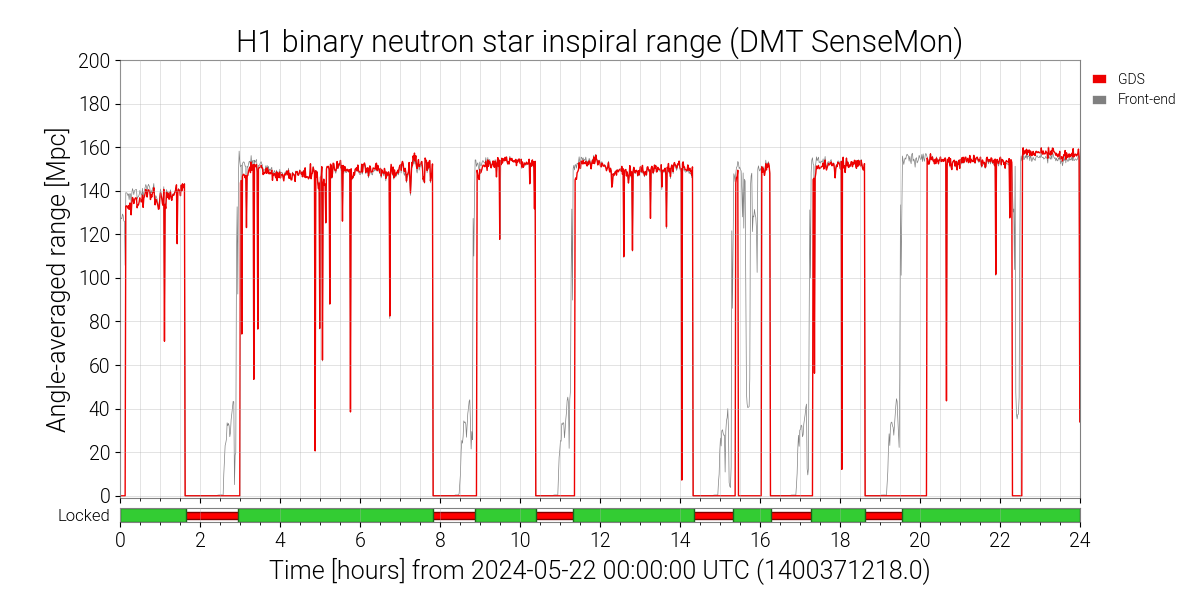
\includegraphics[width=1\linewidth]{images/3_detector_characterisation/may22_bns_range.png}
    \caption{The LIGO-Hanford binary neutron star inspiral range for the 22nd May 2024, created using GWSumm~\cite{gwsumm:2024} and taken from the LIGO Summary Pages-\href{https://summary.ligo.org/}{https://summary.ligo.org/}, please see \href{https://gwosc.org/detector_status/}{https://gwosc.org/detector\_status/} for the public summary pages.}
    \label{3:fig:bns_range}
\end{figure}
%

\subsection{\label{3:sec:noise-transients}Noise Transients}

% Introduction to Noise Transients

Noise transients, commonly referred to as glitches, are short duration bursts of noise found in \gwadj data. The systematic sources of noise described in section~\ref{3:sec:detector-analysis} limit the sensitivity of the detector to a certain frequency range, glitches appear within this sensitivity frequency range. The specific noise transients investigated by detector characterisation are non-Gaussian noise artefacts that have the ability to obscure~\cite{GW170817:2017} or mimic \gwadj signals~\cite{GWMimicking:2010} producing false-alarms in our \gwadj search pipelines. Understanding these glitches is crucial for \gwadj detection, they have the potential to reduce the sensitivity and hinder the reliability of the detectors.
%
% GW170817 Obscured
%

% Characteristics of Noise Transients

There are at least $27$~\cite{gravityspy:2023, gravityspy:2024} different classes of glitch which all manifest with different durations (typically in the millisecond to second range), amplitudes, and glitch morphology. Glitches populate the whole sensitive frequency range of the detectors with some glitches being broadband, affecting up to the whole frequency bandwidth, to others being narrowband and affecting only specific frequency ranges. Glitches are commonly characterised and studied in 2-dimensional time-frequency representations of the one-dimensional strain time series that the detector outputs. The typical time-frequency representation used is the OmegaScan~\cite{qscan:2004} (referred to as `Omega scan' or `Q-scan') which is described later in this chapter.

% Common Sources of Noise Transients

Glitches originate from either environmental sources, instrumental sources or a coupling of the two. As mentioned previously, seismic noise limits the sensitivity of the detectors below ${\sim}10 \, \text{Hz}$, but the coupling of seismic motion into interferometer components can cause one of the more common glitches---\scl. Other environmental noise sources are heavy winds, lightning, and human activity (traffic, construction, trains, the daily commute). A historical glitch identified at LIGO-Livingston was caused by an air conditioning compressor cycling, these glitches were seen by both a magnetometer and the \gwadj strain channel. Other instrumental glitches might be caused by mirror suspensions, electronics, control systems or laser fluctuations.

% Other examples of some common glitches

The most common glitches are: blips~\cite{blips:2019}, \scl~\cite{ArchEnemy:2023} and whistles~\cite{glitschen:2021}, Omega scans of these glitches can be seen in figure~\ref{3:fig:glitches_subset}. The sources of these glitches have been studied, for example, whistles are caused by the beating of radio frequencies in the detector, however, some glitches are from unknown sources such as blips. \Scl has been found from many different sources in the detector and great effort has been made to reduce the presence of \scl in the data~\cite{reducing_scattering:2020} but as of the fourth observing run some \scl still remains.
%
\begin{figure}
    \centering
    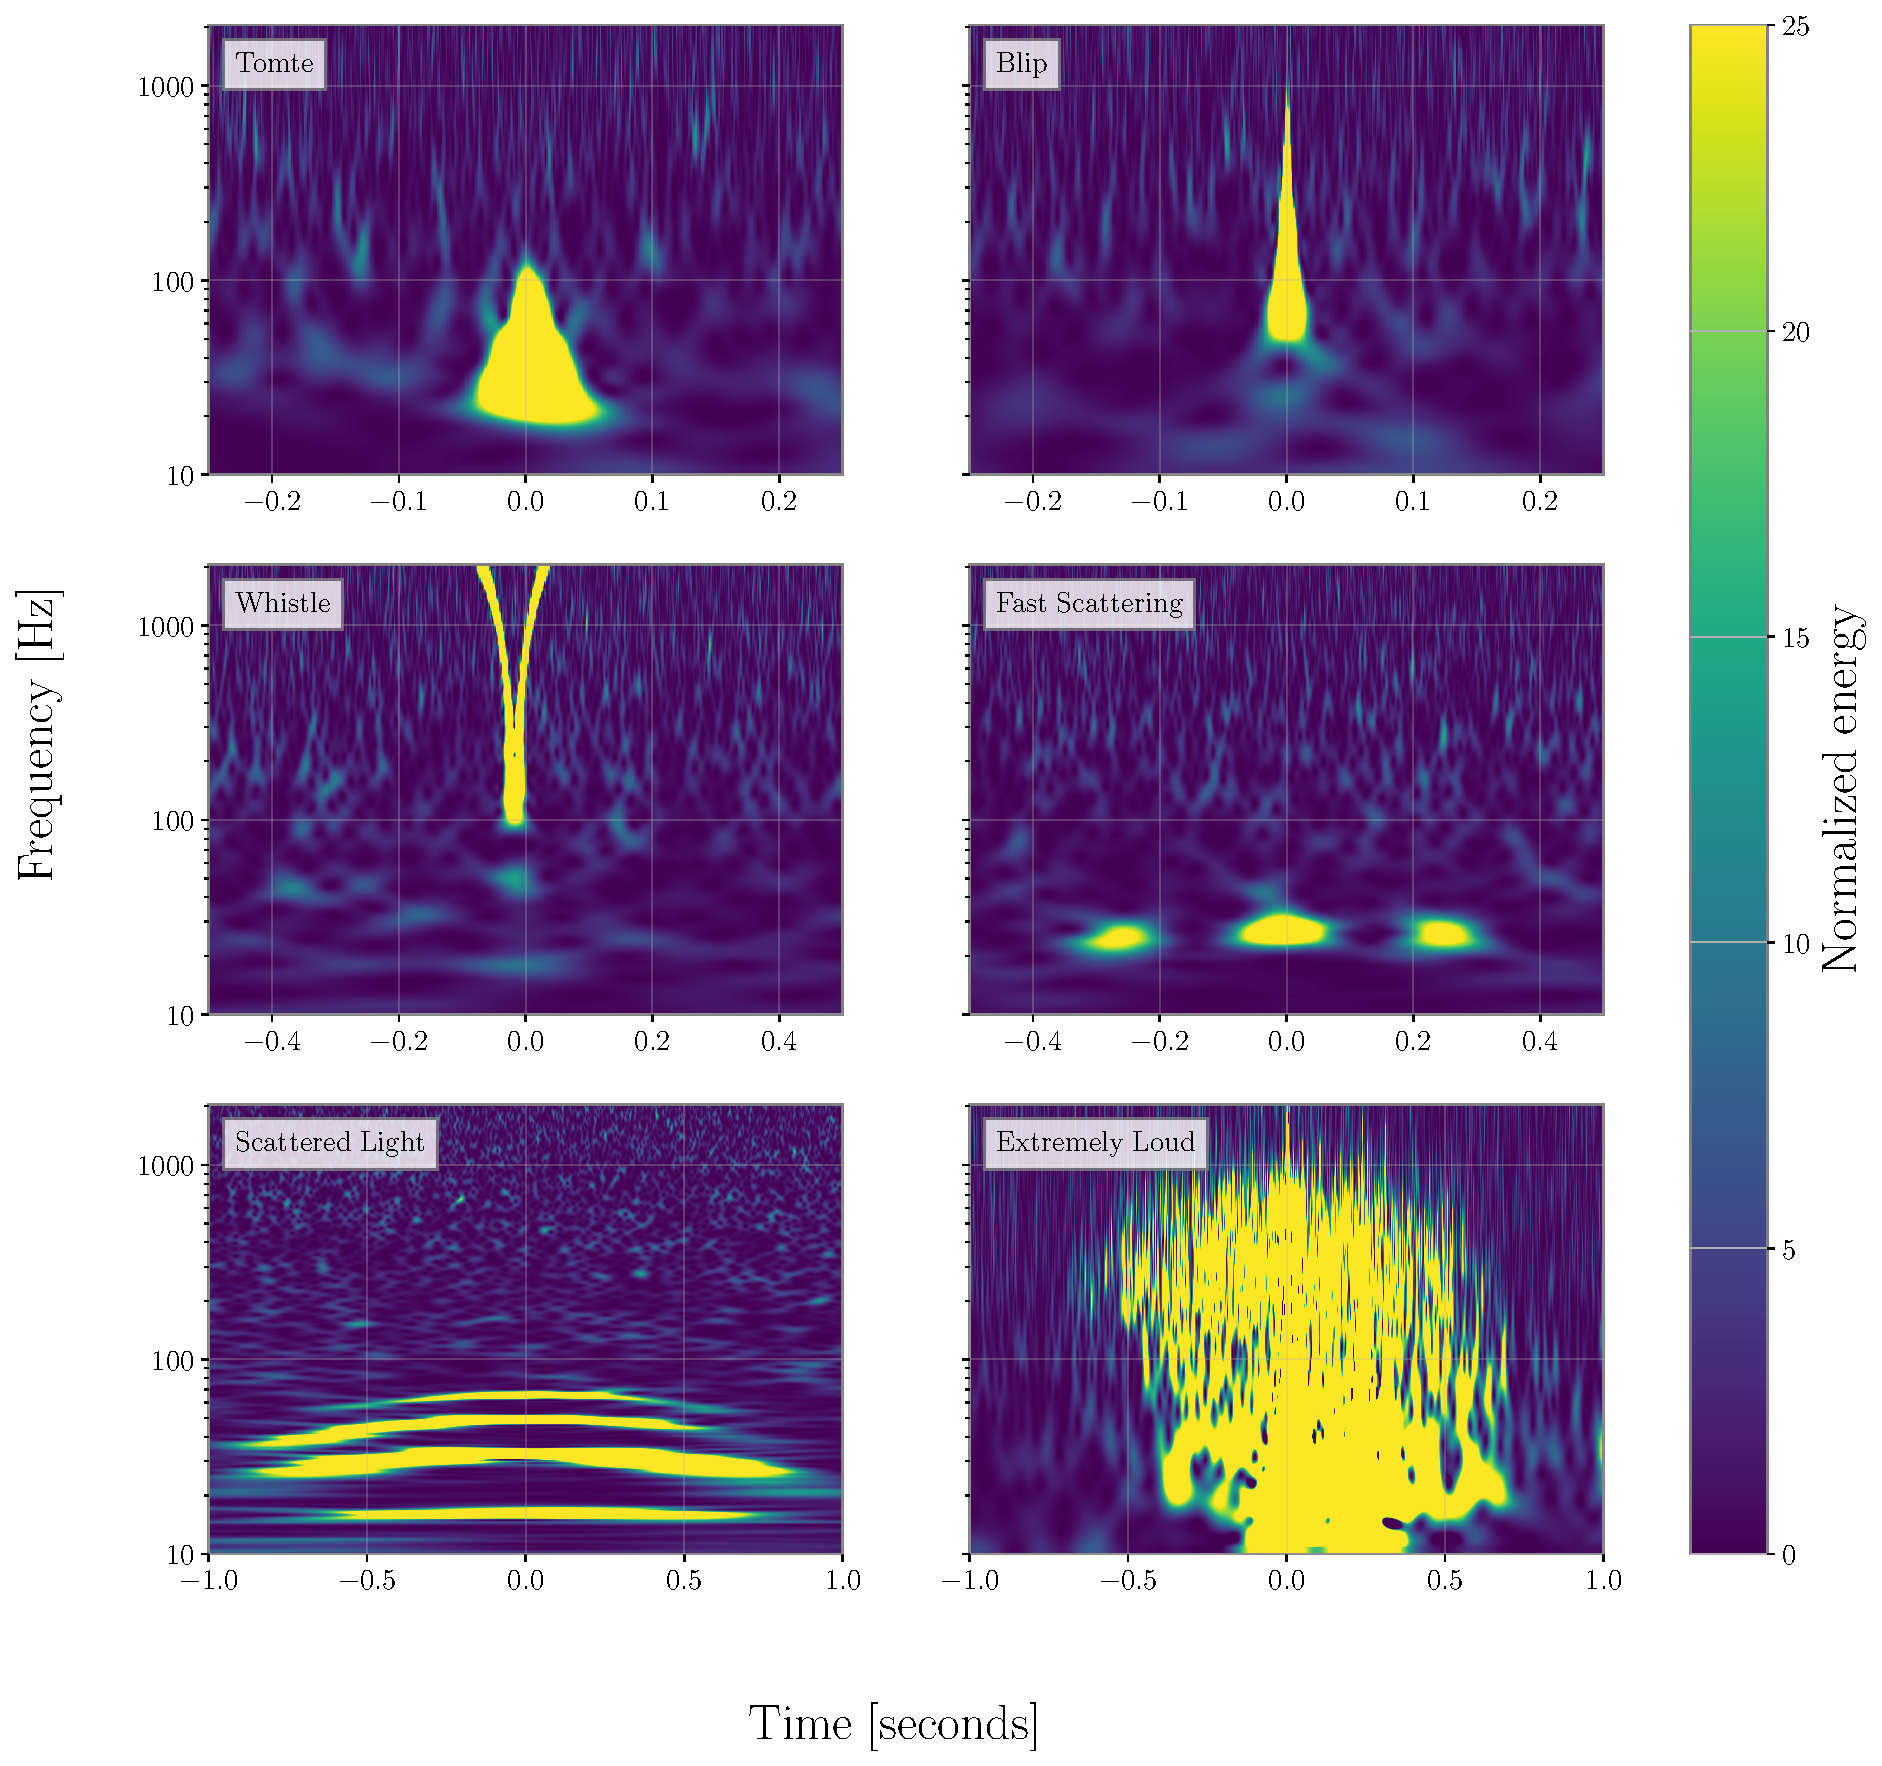
\includegraphics[width=1.0\linewidth]{images/3_detector_characterisation/glitches_subset.pdf}
    \caption{Six classes of glitch commonly found in LIGO detector data. Taken from~\cite{GlitchPlot:2024, gravityspy:2023}.}
    \label{3:fig:glitches_subset}
\end{figure}
%

% Detection and Characterisation of Noise Transients

An number of algorithms and tools have been developed to detect and characterise noise transients in \gwadj data~\cite{ArchEnemy:2023, reducing_scattering:2020, Glanzer:2023, gravityspy:2017, gravityspy:2021, gravityspy:2023, glitschen:2021,  BayesWave:2015, gwadaptive:2022, O3_subtraction:2022, Powell:2016, glitschen:2021}. The primary aim of these tools is the identification of glitches and analysis of properties of the glitches (amplitude, frequency, duration, waveform shape) to determine the source of the noise. Once the noise source has been identified improvements to the detector can be made to eliminate it. Other tools focus on modelling noise transients for the purpose of subtracting them from affected \gwadj data~\cite{ArchEnemy:2023, BayesWave:2015, glitschen:2021, antiglitch:2023}.
%
% GravitySpy figure of a bunch of glitch classes
%

% Auxiliary Channels

Another tool to use in the identification and classification of glitches in the thousands of auxiliary channels alongside the main strain channel~\cite{iDQ:2020} which monitor the many subsystems of the detector and can be used to find noise correlations between the different parts of the instrument~\cite{DQ_vetoes:2017}. The auxiliary channels which are not sensitive to \gws are very useful in identifying any correlations between noise in the gravitational strain channel and noise also seen in another channel which cannot observe \gws, an example of this is the magnetometer recording the same glitch as seen in the \gwadj strain channel when the air conditioning compressor was cycling at LIGO-Livingston~\cite{Nuttall:2018}.

\subsection{\label{3:sec:detchar-tools}Detector Characterisation Tools}

\paragraph{Omega scans}

are two-dimensional time-frequency representations of \gwadj data used very commonly to display \gwadj data in a human interpretable fashion which contains more information that a simple spectrogram and can reveal time-frequency relationships that are virtually impossible for humans to see in the time series. Example Omega scans can be seen in figure~\ref{3:fig:glitches_subset} for a number of glitches.

Detector characterisation uses Omega scans to highlight glitches which can have sharp and localised features in the time-frequency plane. Omega scans calculate the amplitude of strain power at each pixel using the \textit{Q-transform}~\cite{qscan:2004}, where for each point in time and frequency a number of wavelets are created with a varying \textit{quality factor} ($Q$). $Q$ is calculated using
%
\begin{equation}
    Q = \frac{f_{c}}{\sigma_{f}},
\end{equation}
%
where $f_{c}$ is the central frequency and $\sigma_{f}$ is the bandwidth of a wavelet. The bandwidth has a uncertainty relation with the duration, $\sigma_{t}$ of the wavelet
%
\begin{equation}
    \sigma_{t} \sigma_{f} \ge \frac{1}{4\pi},
\end{equation}
%
and so a wider frequency bandwidth will lead to a shorter duration for the wavelet, balanced by the Q-factor. The Q-transform of all these wavelets with the \gwadj strain is taken
%
\begin{equation}
    H(\tau, f, Q) = \int^{\infty}_{-\infty} h(t) w(t - \tau, f, Q) dt,
\end{equation}
%
and the Omega scan algorithm will select the wavelet which produces the greatest amount of power ($|H(\tau, f, Q)|^{2}$) per pixel. As an example, a short-duration glitch (like a blip) would be better tiled with multiple low-frequency bandwidth, high-Q tiles which will resolve the glitch in greater definition than a low-Q tile which captures the whole glitch in one tile.

\paragraph{GravitySpy}

is a citizen science machine learning tool for classifying glitches found in \gwadj data~\cite{gravityspy:2017}. GravitySpy has been trained by volunteers at the project website: at~\href{https://www.zooniverse.org/projects/zooniverse/gravity-spy}{https://www.zooniverse.org/projects/zooniverse/gravity-spy}, hosted on the Zooniverse~\cite{zooniverse}.

GravitySpy has uploaded more than $1.4$ million of Omega scans of \gwadj data which have been found to contain bursts of power which could be caused by glitches. The Omega scans are published on the GravitySpy project and volunteers are given these images and the option for which glitch they think is contained within the image. Once these images have been classified the machine learning algorithm is trained and it can go further to classify the images without the need of volunteers~\cite{gravityspy:2021}.

GravitySpy has been run on data from the second and third observing runs, where it was able to classify 24 different glitch categories. The downsides of GravitySpy are the constantly changing noise background of the \gwadj detectors and the new glitch types emerging which need to be trained on with volunteering again~\cite{gravityspy:2023}.

\paragraph{Data Quality Vetoes}

are used by the \gwadj searches and are a flag applied to periods of data which contain potential data quality issues~\cite{DQ_vetoes:2017}. These periods of data are identified using the ${\sim}200,000$ auxiliary channels~\cite{DQ_vetoes:2017} and when applied to the searches there is a significant reduction in the number of high SNR triggers that would've been found during these times.

The data quality vetoes are constructed using auxiliary channel information which has been found to be strongly correlated to instrumental noise. An example is a significantly elevated transient noise rate in the strain channel five days prior to GW150914~\cite{GW150914:2016} which was traced back to the 45MHz electro-optic modulator driver system used to generate optical cavity control feedback signals~\cite{aLIGO:2015}. The noise caused by this channel was given a category 1 veto data quality flag and removed 2.62\% of the total coincident time from the analysis period.

\paragraph{iDQ}


